\section{Test Examples}
\label{sec:test}

In this section we present few examples that will help the reader to understand 
how this method can be applied to fairly common cases.

\subsection{Example 1: series/parallel configuration}
\label{sec:example1}

The first example is shown in Fig.~\ref{}: it consists of 3 components arranged 
in a series/parallel 
configuration. In this case the following probabilities of failures (on-demand) 
are provided:
\begin{itemize}
  \item $p_A = 1.0 10^{-2}$
  \item $p_B = 5.0 10^{-2}$
  \item $p_C = 1.0 10^{-1}$
\end{itemize}
  
From a dynamic PRA point of view the analysis of this system is performed as follows:
\begin{itemize}
  \item Define 3 stochastic parameters (i.e., $S=3$):
    \begin{itemize}
      \item $s_1$: status of component A
      \item $s_2$: status of component B
      \item $s_3$: status of component C
    \end{itemize}
  \item Assign a distribution to each stochastic parameter; in this case a Bernoulli 
        distribution  
  \item Define $I_i^+$ and $I_i^-$ for each distribution: in this case we have chosen 
        $I_i^-=[0.0,0.1]$ and $I_i^+=[1.0,1.1]$ 
  \item Generate $N$ samples, for example by Monte-Carlo sampling 
  \item Determine $R_0$, $R_i^-$ and $R_i^+$ for each component 
  \item Determine the desired RIMs for each component
\end{itemize}

Note that a Monte-Carlo sampling is not the best sampling strategy in terms of computational 
costs. This is even more relevant if the value of $p_A$, $p_B$ or $p_C$ were several order of 
magnitude lower. 

A more effective sampling strategy would be the Grid sampling: the stochastic variables 
are sampled over a fixed Cartesian grid and a probability weight is associated to each sample. 
In this case, each stochastic variable $s_i$ is sampled over two values, 0.0 and 1.0, and the 
probability weights $w_i^0$ and $w_i^1$ values associated to each sample coordinate are:
\begin{itemize}
  \item $s_i=0.0$: $w_i^0=prob(s_i \in [-\infty,0.5])$
  \item $s_i=1.0$: $w_i^1=prob(s_i \in [0.5,+\infty])$
\end{itemize}
Following this grid sampling strategy, only $2^N=8$ are needed.
Below, the FV importance for all three components obtained by RAVEN (using a Grid sampling 
strategy) are shown compared with the analytical ones.

\begin{table}
  \caption{Results obtained for Example I.} 
  \centering 
  \begin{tabular}{c | c | c } 
    \hline 
     & Analytical & RAVEN \\ 
    \hline 
    $FV_A$ & 0.6656 & 0.6656   \\
    $FV_B$ & 0.3311 & 0.3311   \\
    $FV_C$ & 0.3311 & 0.3311   \\
    \hline 
  \end{tabular}
  \label{tab:example1} 
\end{table}

\subsection{Example 2: Time-dependent system}
\label{sec:example2}

The second example is similar to Example I but with different reliability data: 
a failure rate is provided for each component (mission time: 24 hours): 
\begin{itemize}
  \item $\lambda_A = 1.0 10^{-3} hr^{-1}$
  \item $\lambda_B = 5.0 10^{-3} hr^{-1}$
  \item $\lambda_C = 1.0 10^{-2} hr^{-1}$
\end{itemize}
Thus it is assumed that failure probability of each component is exponentially 
distributed: sampled value $s_i$ from its own distribution is failure time of each 
component ($t_A$, $t_B$ and $t_C$).
In this case, $I_i^+$ and $I_i^-$ can be defined as follows:
\begin{itemize}
  \item $I_i^-=[24.0,+\infty]$: component is considered perfectly reliable if the failure 
        time is greater than the mission time
  \item $I_i^+=[0.0,1.0]$: component is considered unreliable if the failure time 
        occurs within the first hour
\end{itemize}

As shown for Example I, a Grid sampling strategy has been employed. Table~\ref{} shows the 
FV importance for all three components obtained by RAVEN (using a Grid sampling strategy) 
compared with the analytical ones.

\begin{table}
  \caption{Results obtained for Example II.} 
  \centering 
  \begin{tabular}{c | c | c } 
    \hline 
     & Analytical & RAVEN \\ 
    \hline 
    $FV_A$ & 0.48957 & 0.48957  \\
    $FV_B$ & 0.4983  & 0.4983   \\
    $FV_C$ & 0.4983  & 0.4983   \\
    \hline 
  \end{tabular}
  \label{tab:example2} 
\end{table}

\subsection{Example 3: stand-by configuration}
\label{sec:example3}

The third example considers a simplified ECCS model (see Fig.~\ref{}) for a Pressurized 
Water Reactor (PWR). It consists of the following components and for a subset of them a 
value of mean time to failure (MTTF) is provided:
\begin{itemize}
  \item Motor-operate valve M (MTTF = 24 h)
  \item Two redundant pumps, pump1 and pump2 (MTTF = 12 h)
  \item Heat exchanger HX (reliability = 1.0)
\end{itemize}

Pump1 is normally used while pump2 is on standby. If Pump1 fails then pump2 provide water flow. 
Pump2 cannot fail while in standby. Switch from pump1 to pump2 is perfectly reliable. 
The cooling is such that it takes 2 hours to reach vessel failure condition if the M-pump1-pump2 
system has failed. Top event is: overheating of the vessel. Mission time is again equal to 24 hours.

Failure of the system occurs when temperature insider the core reaches a limit temperature. 
Note that the configuration is slightly different from the one presented in the first two 
examples (here a stand-by configuration is introduced) but also the condition of system failure 
is dictated by the dynamic behavior of the PWR.  The system is designed such that a late failure 
of the ECCS may not lead to system failure (i.e., natural circulation is providing enough cooling). 
In other words, the ECCS is vital especially in the hours right after a reactor scram.

\begin{figure}
    \centering
    \centerline{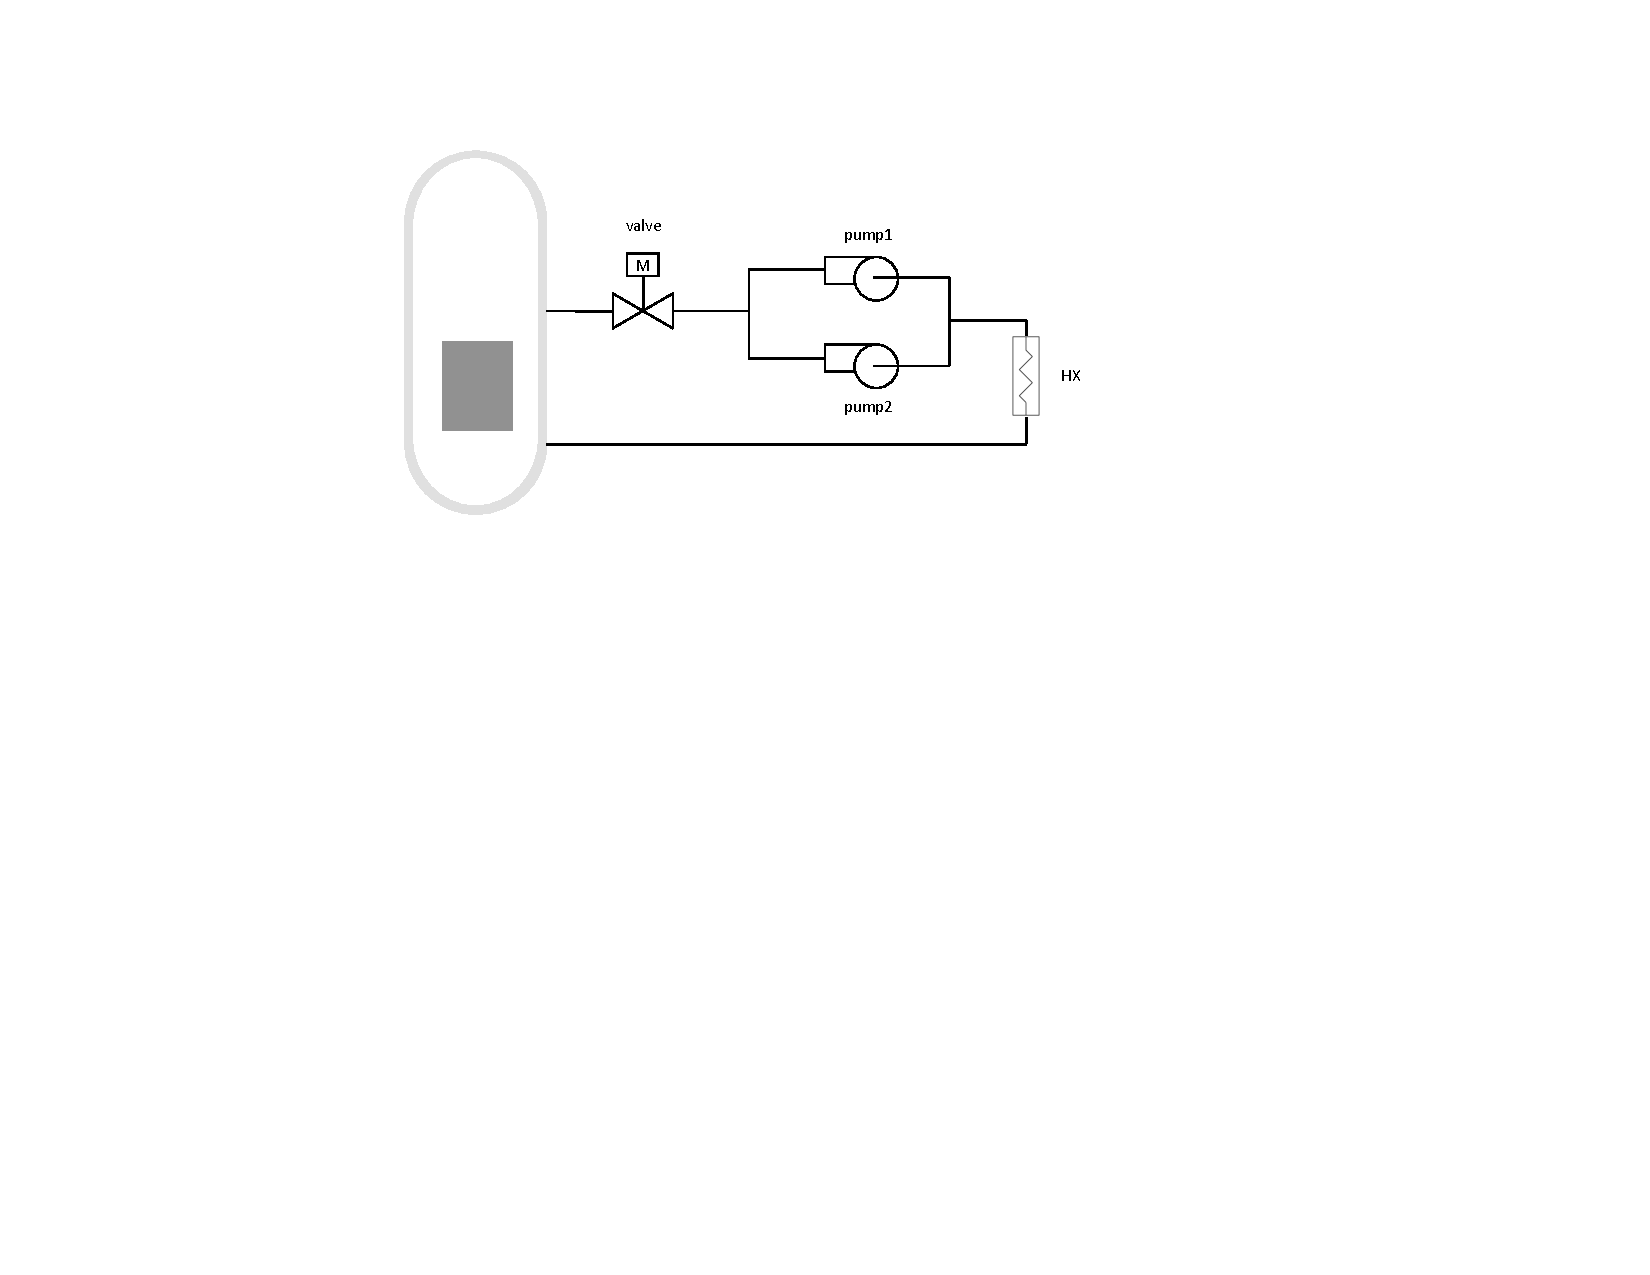
\includegraphics[scale=0.6]{case2.pdf}}
    \caption{System for Example III.}
    \label{fig:example3}
\end{figure}

Note in this case classical PRA methods require few model simplifications in order to correctly 
determine system reliability.
In contrast, a dynamic PRA analysis follows the same steps presented for the first two examples; 
the only difference is represented by the simulator that is actually employed.
Below are shown the FV importance for all three components obtained by RAVEN (using a Monte-Carlo 
sampling strategy) compared with the analytical ones.

\begin{table}
  \caption{Results obtained for Example III.} 
  \centering 
  \begin{tabular}{c | c | c } 
    \hline 
     & Analytical & RAVEN \\ 
    \hline 
    $FV_{pump1}$ &   & 0.25893  \\
    $FV_{pump2}$ &   & 0.25893   \\
    $FV_{valve}$ &   & 0.30331   \\
    \hline 
  \end{tabular}
  \label{tab:example3} 
\end{table}

\subsection{Example 4: $K$ out of $N$ configuration}
\label{sec:example4}

\begin{figure}
    \centering
    \centerline{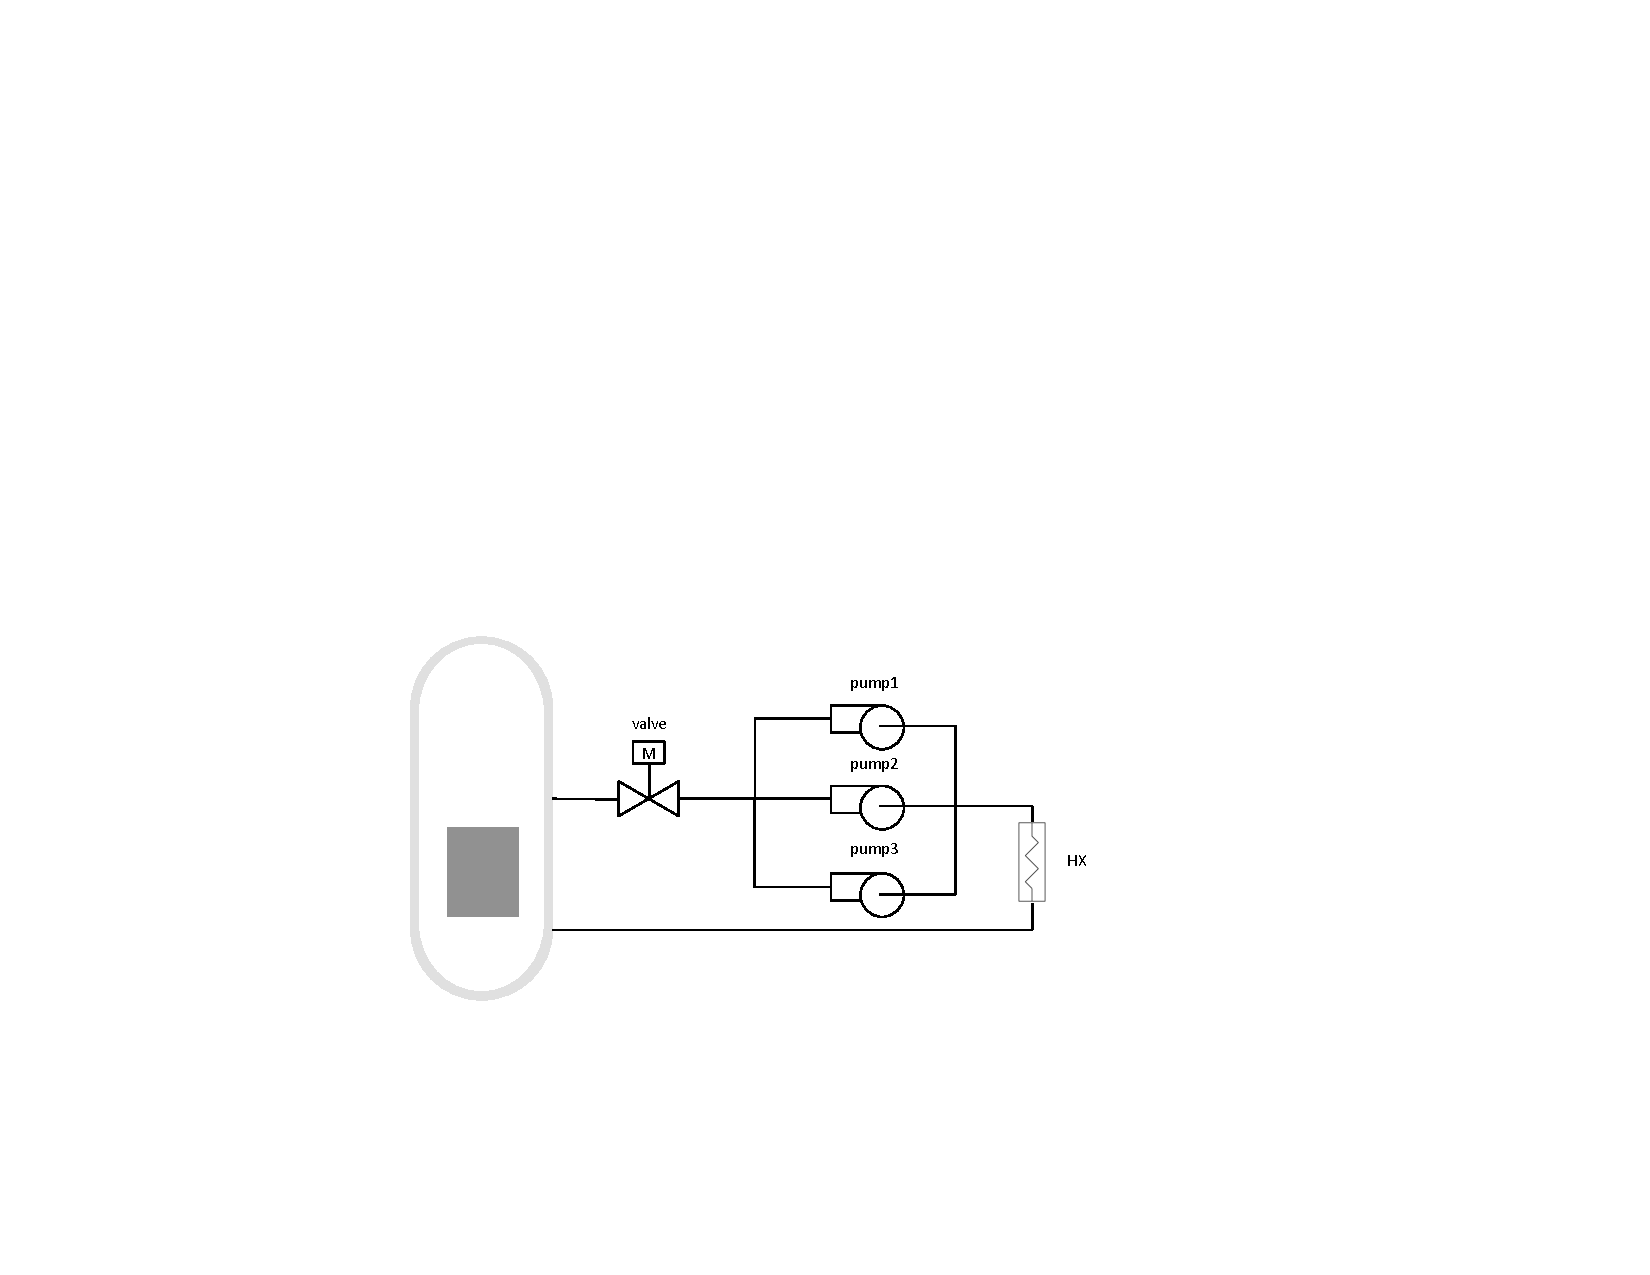
\includegraphics[scale=0.6]{case3.pdf}}
    \caption{System for Example IV.}
    \label{fig:example4}
\end{figure}
